\chapter{Structure of CoCos}

This chapter explains the nature of a new member in the family of hybrid securities; so-called contingent convertibles (CoCos). In the following, the general structure of these new instruments will be explained (section \ref{definitioncocos}) including characteristic design features among others their trigger (section \ref{triggermechanism}) and loss-absorption mechanism (section \ref{lossabsorption}).

\section{Definition}\label{definitioncocos}

CoCos are hybrid financial instruments with automatic conversion mechanisms that morph debt into equity when the financial soundness of the issuer is at stake. In such a case, a predefined trigger event occurs. For instance, a regulatory capital ratio falls below a predefined threshold. That said, a write-down of the notional of the CoCo is also a viable loss-absorption mechanism. \citep{de2011pricing} Figure \ref{figure:anatomy} provides a good overview of the previously mentioned design characteristics. All anatomic aspects will be further explained in the subsequent sections.\\

\begin{figure}[ht]
	\centering
	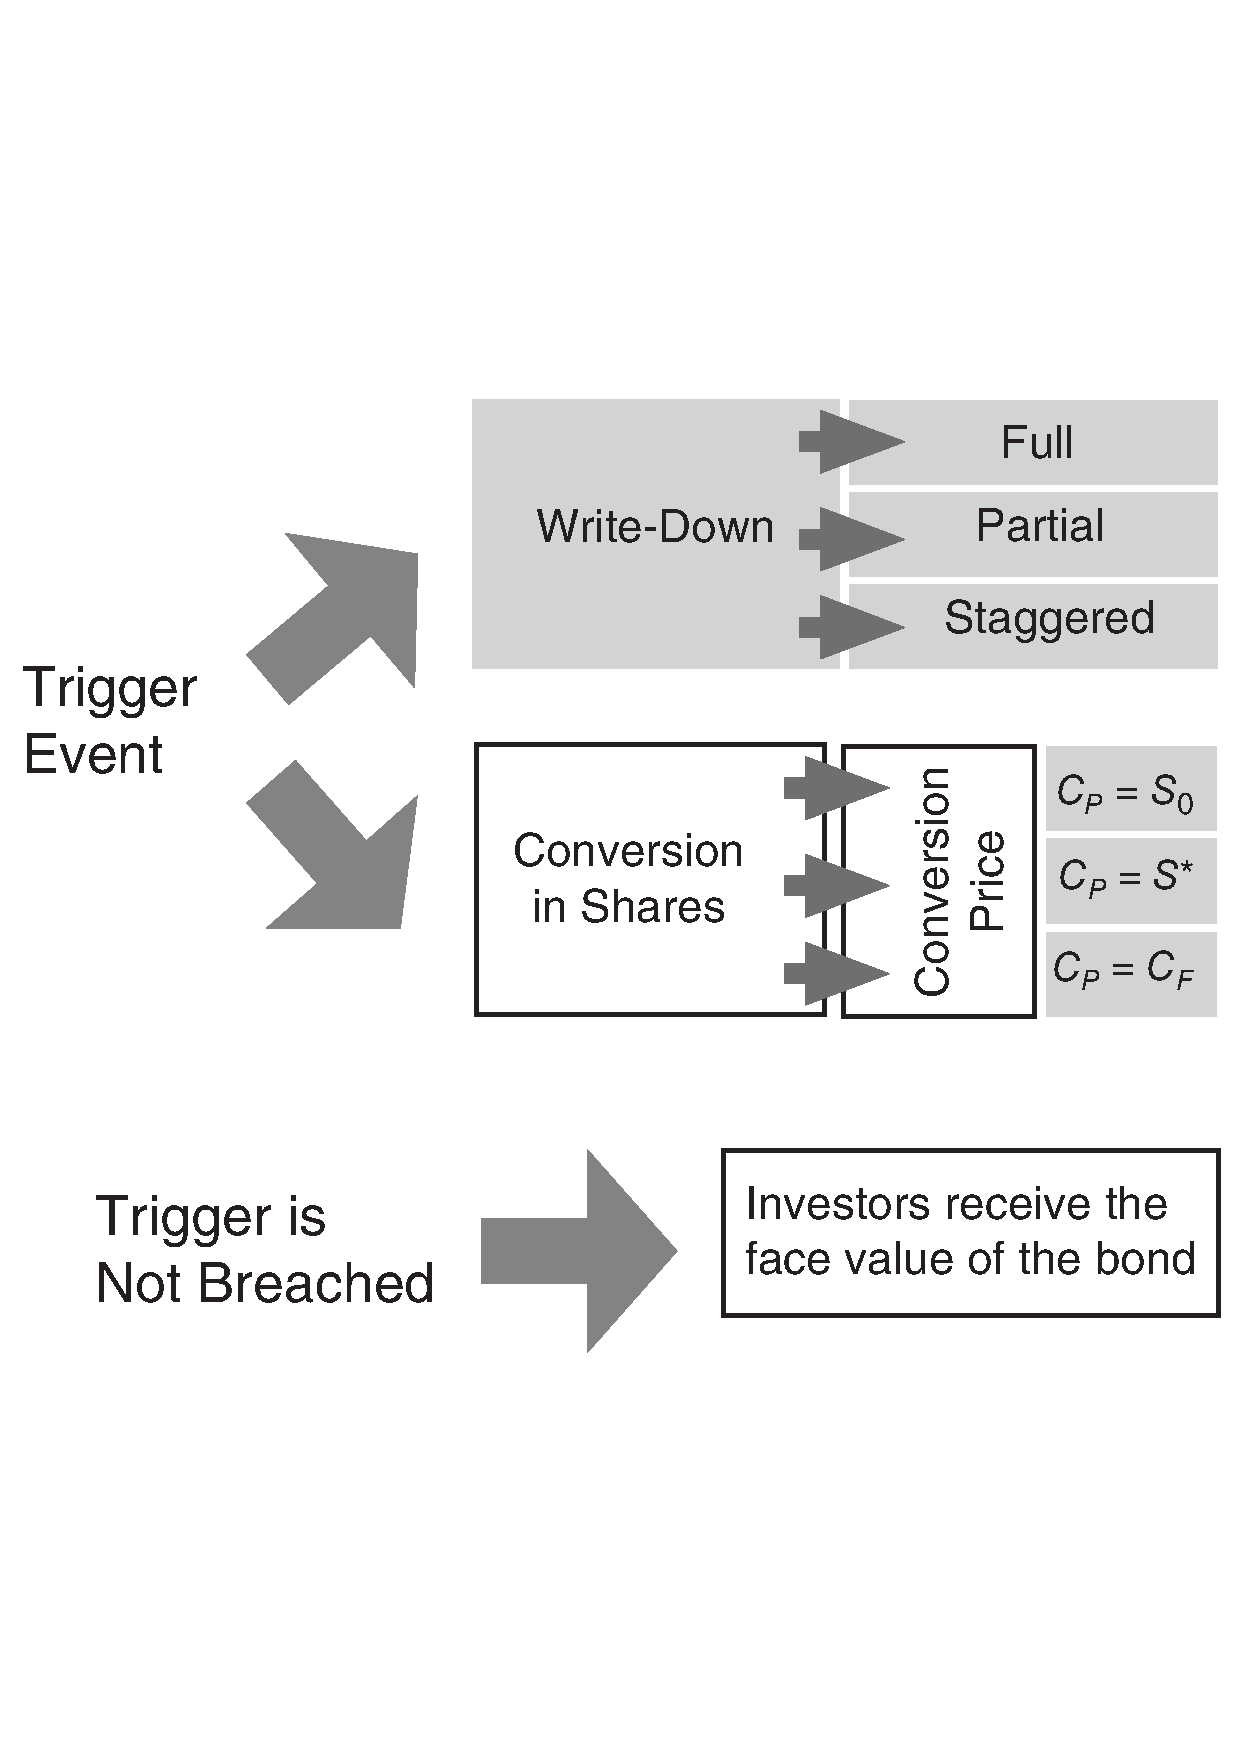
\includegraphics[trim=0.6cm 7.05cm 0.9cm 7cm, scale = 0.4]{media/anatomy} \par
	\caption[Anatomy of CoCos]{Anatomy of CoCos \citep{de2014handbook}}
	\label{figure:anatomy}
\end{figure}

CoCos are particularly interesting from the perspective of a regulatory authority because they might mitigate externalization costs of insolvencies and frictions due to spill-over effects. In times of distress, stakeholders might question the financial viability of the respective financial institute. However, a distressed bank does not have to approach new investors to issue new capital in extremely though times as everything happens automatically.\citep{de2011pricing}\\ 

In 2009, the Lloyds Banking Group was the first financial institute to issue this new financial instrument. They offered hybrid debt holders to swap their holdings into CoCos.\citep{de2011pricing} In 2010, the Basel Committee on Banking Supervision (BCBS) provided further impetus to the use of this instrument when it disclosed its proposal to ensure the loss absorbency of regulatory capital at the point of non-viability. The general argumentation of the BCBS is that regulatory capital instruments have to be capable of absorbing financial losses in gone-concern phases.\citep{basel2010proposal}.

%\begin{figure}[ht]
%	\centering
%	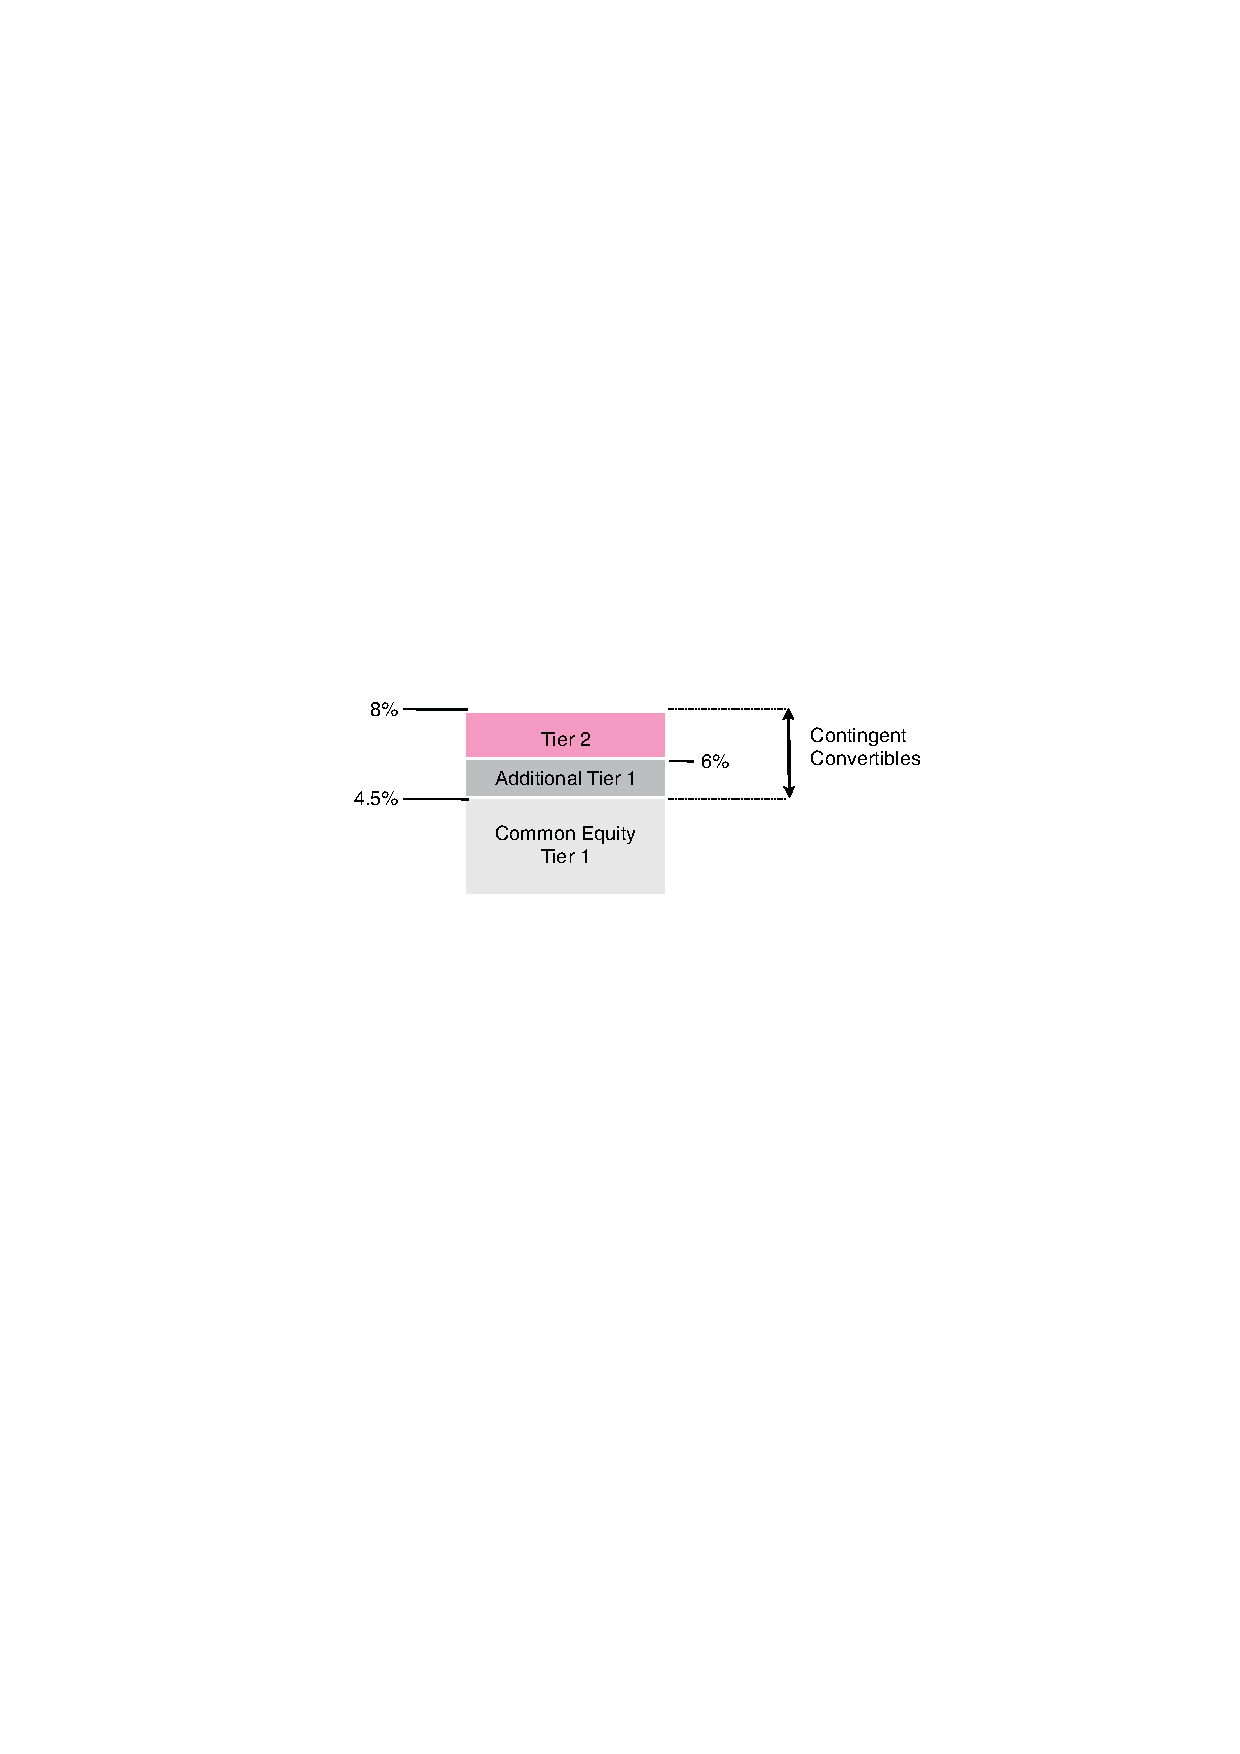
\includegraphics[trim=0.1cm 0.1cm 0.2cm 0.1cm, scale = 1]{media/basel3} \par
%	\caption[CoCos under Basel III]{CoCos under Basel III \citep{de2014handbook}}
%\end{figure}

%The term CoCo is used to describe a new type of convertible bond that is automatically converted into a predetermined amount of shares when a predefined trigger is breached. Since this type of bond is transformed into equity upon conversion, it would be available for further loss-absorption and therefore satisfies the new regulatory requirements of hybrid capital instruments. \citep{zahres2011contingent}

\section{Trigger Mechanism} \label{triggermechanism}

The trigger is a key design element of a CoCo. In the following section, four different trigger mechanisms will be evaluated based on general design criteria as summarized by \citet{erismann2015pricing}. The concept of an accounting trigger will be illustrated in section \ref{accountingtrigger} followed by the market trigger in section \ref{markettrigger}. Additionally, the regulatory trigger will be detailed in section \ref{regulatorytrigger} and the multi-variate trigger will be explained in section \ref{multivariatetrigger}. Hereinafter, the trigger types will be evaluated based on the following criteria:

\begin{itemize}
\renewcommand\labelitemi{--}
\item \textbf{Clarity}:  The trigger mechanism should be universally applicable irrespective of the jurisdiction in which the CoCo is traded.
\item \textbf{Fixedness}: The definition of a CoCo's trigger should remain the same until maturity.
\item \textbf{Frequency}: Data to which the trigger is linked should be updated at frequent intervals.
\item \textbf{Objectiveness}: The trigger mechanism should be based on observable and well-known facts. Their should be no room for subjectivity.
\item \textbf{Publicity}: Data should be open to the general view of all market participants. This needs to be possible without concealment. 
\item \textbf{Transparency}: The trigger mechanism should have the property that investors can see it publicly, thereby reducing the chance of manipulation.
\end{itemize}

\subsection{Accounting Trigger}\label{accountingtrigger}

CoCos with accounting trigger have a loss absorption mechanism which is inherently connected to the financial soundness of a bank's balance sheet. Accounting triggers are built upon capital ratios which compare a bank's regulatory capital with its assets. Conversion occurs if a pre-determined metric falls below a certain threshold. Hence, capital ratios are an objective indicator for a bank's solvency as they are defined uniformly for all financial institutions by regulatory authorities. \citep{de2014handbook} \citet{pazarbasioglu2011contingent} note that accounting triggers are easy to price, intuitive and simple to implement. Issuing banks and regulators seem to have perceived the benefits of accounting triggers partly because a significant portion of CoCos use the common equity tier (CET1) ratio as reference metric. Examples of CoCos will be described shortly in section \ref{examples}.\\

That said, objections against accounting triggers follow the line of thought that they just become active long after the need for loss absorbing capital arose. One might argue that accounting triggers assess the viability of financial institutions from a perspective that is far-removed from reality. \citep{de2011pricing} Moreover, as accounting concept, book values are prone to manipulation and managerial dishonesty especially in times of distress. \citep{mcdonald2013contingent}\\ 

Empirical findings bring up a further aspect. \citet{haldane2011capital} points out that major financial institutions, which either went bankrupt, were bailed out or were taken over under distress during the global financial crisis, reported similar CET 1 ratios right before the collapse of Lehman Brothers compared to their peers which coped relatively well with the collapse of the financial system. In this context, \citet{haldane2011capital} highlights that market-based solvency measures\footnote{\citet{haldane2011capital} mentions three metrices: (1) market-based capital ratio (ratio of market capitalization to total assets), (2) market-based leverage ratio (ratio of market capitalization to total debt) and (3) Tobin's Q (ratio of market capitalization to book value of equity).} performed creditably as they showed clear signals of impending distress a year ahead of the bankruptcy of Lehman Brothers. Empirical evidence of \Citet{valukas2010report} further supports these findings. This leads to the conclusion that CoCos with accounting triggers might not reinforce distressed banks at the right time but instead produce more false positives, which means that CoCos of non-distressed banks trigger prematurely. Inefficiencies like higher funding costs could be the consequence. \citep{pazarbasioglu2011contingent}

\subsection{Market Trigger} \label{markettrigger}

A market trigger uses directly observable indicators like the issuing company's share price or credit default swap (CDS) spreads while assuming sufficiently efficient markets. The major advantage of those measures is that one can observe and verify them in real-time. \citep{haldane2011capital} Market triggers are widely discussed in academia and seen as preferable trigger mechanism. \citet{calomiris2013design} pronounce themselves for using share prices. Besides, \citet{haldane2011capital} and \citet{pazarbasioglu2011contingent} contend to apply market-based capital ratios as trigger indicator. Their line of argumentation is based on some of the best-known examples of corporate defaults, which were indicated well before by a serious and continuous deterioration of a company's market capitalization.\\ 

This also applies to the aforementioned example of Lehman Brothers. If the bank had been obliged to issue CoCos with a trigger directly linked to its share price the decline in equity value would have triggered the conversion in due time.\citep{calomiris2013design} Hence, the bankruptcy could have been prevented with a CoCo. However, practitioners argue that it comes at a risk to use market data as reference because markets are prone to manipulation. Moreover, self-fulfilling prophecies of share price dilution could lead to downward spirals that ultimately lead to CoCo conversions. \citep{pazarbasioglu2011contingent} The severity of the aforementioned argumentation can be attentuated by using moving averages, which are less susceptible to manipulation. 

\subsection{Regulatory or Non-Viability Trigger} \label{regulatorytrigger}

Regulatory or non-viability trigger is a conversion mechanism by which a CoCo is converted into equity at the discretion of the responsible supervisory authority. The rationale behind this approach is that regulators want to limit the impact of any development that could pose a danger to the going-concern of a systemically important bank.\citet{erismann2015pricing} Moreover, this kind of trigger would eliminate the periodicity problem of accounting data and the risk of market manipulation.\\ 

Though, it is very difficult for market participants to estimate the conversion probability of a CoCo with regulatory trigger. The valuation of such a hybrid instrument becomes opaque for market participants with limited information. \citep{alvemar2012modelling} One can also argue that a CoCo's marketability is weakened because of the greater uncertainty which could ultimately lead to higher funding costs. \citep{de2014handbook} 

\subsection{Multi-Variate Trigger} \label{multivariatetrigger}

The multi-variate trigger uses a combination of the aforementioned trigger mechanisms. It extends the accounting trigger of a CoCo by a universal regulatory trigger which covers severe states of the world adversely impacting the stability of the financial system. In this context, the \citet{squam2009expedited} supports the implementation of this dual trigger mechanism as it combines the best of two worlds. On the one hand, the bank-specific trigger serves as disciplining mechanism for a bank's management. It reduces the political pressure from the regulator who has to decide whether the systemic trigger is met. Second, if the conversion of a CoCo is only linked to a systemic trigger, even well capitalized banks would be forced to convert debt into equity during a systemic crisis. This would disincentivize financially sound banks to preserve their status quo.

\subsection{Evaluation of Trigger Types}
Generally, one can evaluate the aforementioned trigger types based on the design criteria as stated in the beginning.

\begin{table}[H]
	\setlength{\extrarowheight}{2.5pt}
	\centering
	\begin{tabular}{lcccc}
		\toprule
			 & Accounting & Market & Regulatory & Multi-Variate \\
		\midrule
			Clarity & \cellcolor{yellow!20} medium & \cellcolor{green!20} high & \cellcolor{red!20} low & \cellcolor{yellow!20} medium\\
			Fixedness & \cellcolor{green!20} high & \cellcolor{green!20} high & \cellcolor{red!20} low & \cellcolor{green!20} high \\
			Frequency & \cellcolor{yellow!20} medium & \cellcolor{green!20} high & \cellcolor{red!20} low & \cellcolor{green!20} high\\
			Objectiveness & \cellcolor{yellow!20} medium & \cellcolor{green!20} high & \cellcolor{red!20} low & \cellcolor{yellow!20} medium \\
			Publicity & \cellcolor{green!20} high & \cellcolor{green!20} high & \cellcolor{green!20} high & \cellcolor{green!20} high \\
			Transparency & \cellcolor{yellow!20} medium & \cellcolor{green!20} high & \cellcolor{red!20} low & \cellcolor{yellow!20} medium \\
		\bottomrule
	\end{tabular}
	\caption[Evaluation of different trigger mechanisms]{Evaluation of different trigger mechanisms based on design criteria. The status high means that the trigger type meets the requirements, whereas low implies that it does not satisfy the conditions. \citep{erismann2015pricing}}
	\label{table:evaluationtrigger}
\end{table}

We see in table \ref{table:evaluationtrigger} that the market trigger is a preferable mechanism as it fulfills all important design criteria. Furthermore, one has to take into account that \citet{haldane2011capital} described that market trigger were historically the preferable mechanism as it served as early-warning indicator. In section \ref{examples} different CoCos will be highlighted with their design elements also covering their trigger mechanism. This is a good way to understand whether banks and regulators followed the aforementioned rationale.

\section{Loss-Absorption Mechanism} \label{lossabsorption}

As mentioned before, banks can decide whether they want to issue CoCos with equity conversion or with a haircut on the notional. 

\subsection{Conversion into Shares}
The number of shares which a CoCo holder receives at conversion is given by the conversion rate $C_r$. This figure is specified ex-ante and the conversion into shares gives an investor in case a certain trigger threshold is breached. Besides, the conversion amount $\alpha N$ is determined by the conversion fraction $\alpha$ and the notional $N$. One can now derive the implied conversion price $C_p$ with the following formula. \citep{de2014handbook}
\begin{align}
C_p &= \frac{\alpha N}{C_r}
\end{align}

The recovery rate $R_{CoCo}$ can be calculated based on the share price $S^*$ at the trigger event and the conversion price $C_p$. One might recognize that a CoCo holder is better off if $C_p$ is low because the recovery rate $R_{CoCo}$  will be higher as more equity will be created. 
\begin{align} \label{recoveryrate}
R_{CoCo} &= \dfrac{S^*}{C_p}
\end{align}

If the CoCo is converted into shares one can directly derive the loss $L_{CoCo}$ a CoCo holder has to bear.
\begin{align}
{Loss}_{CoCo} &= N - C_r S^* = N - (1 - R_{CoCo}) = N \left(1 - \frac{S^{*}}{C_p} \right)
\end{align}

Generally, the final payoff $V^{CoCo}$ which an investor receives at maturity $T$ is given by:
\begin{align}\label{valueatmaturity}
    V^{CoCo}_T &= \begin{cases} N & \text{if not triggered} \\ (1 - \alpha) N + \frac{\alpha N}{C_p} S^{*} & \text{if triggered} \end{cases}
\end{align}

\subsubsection*{Floating conversion price}l
At issuance one can set a floating conversion price where $C_p$ is equal to $S^*$. $S^*$ is the share price which is observed at the trigger event. Intuitively, the value of the share price at trigger time $t$ is low as the purpose of the CoCo is to help undercapitalized banks in tough times. If the issuer chooses to set the conversion price at this specific level the recovery rate of a CoCo holder is $100\%$ whereas the current shareholders carry the load of conversion. Regulators would not categorize this instrument to be adequate as regulatory capital instrument as the dilution is potentially unbounded and it is effectively not loss absorbing. \citep{de2014handbook}

\subsubsection*{Fixed conversion price}
Fixed conversion means that the conversion price $C_p$ is equal to the share price of the issue date $S_0$. On the one hand, this means that the amount of shares upon conversion is fixed at the date of issue and one the other hand, the amount is known beforehand. This is in contrast to the floating conversion price where there was no limit on the amount of shares converted.\citep{de2014handbook}

\subsubsection*{Floored conversion price}
One can also specify a floored conversion price where $C_p$ is equal to $\max\left( S^*, S_F \right)$. Hence, the conversion price $C_p$ is either equal to the floored share price $S_F$ or to the share price $S^*$, which is observed at the triggering event. It is a compromise between the floating and fixed conversion price as stated before. \citep{de2014handbook}

\subsection{Write-Down}

The implementation of a loss-absorption mechanism with equity conversion entails several disadvantages which might reduce the marketability of a CoCo. For instance, portfolio managers with a mandate to invest in corporate bonds may face hard times to broaden their investment universe because CoCos with equity conversion mechanism may be converted into shares. Furthermore, the write-down feature is preferable as investors know beforehand the potential loss. Shareholders might be concerned that their voting rights are diluted when a conversion occurs. Both investors and shareholder have clear incentives to influence a bank to issued CoCos with write-down mechanism.  

\subsubsection*{Full write-down}
The first way is to specify a full write-down of a CoCo's face value in case a certain capital ratio drops below a predetermined level.

\subsubsection*{Partial write-down}
Another approach is that only a certain portion of the notional is wiped out. 

\subsubsection*{Staggered write-down}
The third option consists of a staggered write-down. This means that a CoCo inherits a flexible write-down mechanism. Losses materialize up to the point to enhance a certain capital ratio to a fixed threshold. One might think of a gradual process in which a haircut is imposed in multiples of $10\%$.


\chapter{CoCo Examples} \label{examples}

For each of the aforementioned loss-absorption mechanisms selected CoCos are characterized hereinafter to gain a better sense of how these hybrid products are implemented in real-life. To that end, broadly discussed CoCos of well-known financial institutions are picked out, i.a. Lloyds, Credit Suisse, Barclays, Rabobank and Zurich Cantonal Bank.
\begin{table}[H]
	\tiny
	\setlength{\extrarowheight}{2.5pt}
	\centering
	\begin{tabular}{p{1.5cm}p{2cm}p{2cm}p{2cm}p{2cm}p{2cm}}
		\toprule
			& Lloyds & Credit Suisse & Barclays & Rabobank & Zurich Cantonal Bank \\ 
		\midrule
			Full Name & Enhanced Capital Notes & Tier 2 Buffer Capital Notes & Contingent Capital Notes & Senior Contingent Notes & Subordinated Tier 1 Notes \\
			ISIN & XS0459088281 & XS0595225318 & US06740L8C27 & XS0496281618 & CH0143808332 \\
			Issue Date & Dec 1, 2009 & Feb 24, 2011 & Nov 21, 2012 & Mar 19, 2010 & Jan 31, 2012 \\ 
			Maturity & May 12, 2020 & Feb 24, 2041 & Nov 21, 2022 & Mar 19, 2020 & Perpetual \\ 
		\midrule
			Nominal & GBP 7.5 bn  & USD 2 bn & USD 3 bn & EUR 1.25 bn & CHF 590 mn\\
			Callability & n/a & Callable from Aug 24, 2016 & n/a & n/a & Callable from Jun 20, 2017 \\	
			Coupon & 7.5884\% & 7.875\% & 7.625\% & 6.875\% & 3.5\% \\
		\midrule
			Write-down & n/a & n/a & Full by (100\% of notional) & Partial (75\% of notional) & Staggered (multiples of 25\% of notional) \\
			Conversion price & Fixed at GBP 0.59 ($=S_0$) & Floored at lowest of USD 20 and 30 day-VWAP & n/a & n/a & n/a \\
			Trigger & Core Tier 1 capital ratio & CET 1 ratio & CET 1 ratio & Equity capital ratio (Member certificates to risk weighted assets)& CET 1 ratio \\
			Trigger Level & 5\% & 7\% & 7\% & 7\% & 7\% \\
		\bottomrule
	\end{tabular}
	\caption[CoCo examples with different loss-absorption mechanisms]{CoCo examples with different loss-absorption mechanisms \citep{lloyds2009, creditsuisse2011, barclays2010, rabobank2010, zkv2013}}
	\label{tbl:examples}
\end{table}

An overview of CoCos which have different characteristics with respect to their loss-absorbency can be found in table \ref{tbl:examples}. The first two apply similar equity conversion mechanisms whereas the latter three use different write-downs.

\section{Lloyds -- Enhanced Capital Notes}
In 2009, Lloyds issued Enhanced Capital Notes (ECN)  in the amount of GBP 9 bn in an debt exchange offer. At that time, the company was the first bank to refinance itself with CoCos. The ECN inherit an accounting-based trigger which is disclosed each quarter. These instruments convert into equity should the bank's Core Tier 1 capital (Basel II) fail to remain above the threshold of 5\%. If this is the case, the conversion mechanism morphs the entire face value to a fixed amount of ordinary shares. But today, banks in the UK move to Basel III. Yet, this leads to stricter definitions of risk-weighting compared to Basel II. Thus, the initial threshold of 5\% Core Tier 1 capital ratio is not sufficient as it translates to a significantly lower CET 1 ratio under Basel III. Regulators believe that the ECN might not buttress the balance sheet in times of stress. Hence, the supervisory authorities did not consider them in their latest stress tests. Subsequently, Lloyds has started to call in the CoCos. \citep{lloyds2009}

\section{Credit Suisse -- Tier 2 Buffer Capital Notes}
The rationale of Credit Suisse's issue of its Tier 2 Buffer Capital Notes (T2BCN) in 2011 follows the recommendation of the Swiss Commission of Experts. Their goal is to establish measures which further solidify the capital structure of the Swiss banking sector. In this context, CoCos play an important role for Credit Suisse in strengthening its capital base to 19\% until 2019.  In order to achieve the given objectives, USD 2 bn in T2BCN have been raised with a coupon of 7.875\%. The trigger event is specified to convert the T2BCN into ordinary shares if the reported risk-based capital ratio is below 7\%. The conversion price is floored at the average daily share price of the last 30 days or USD 20. It may also be that the CoCo is converted if the FINMA determines that Credit Suisse needs to be bailed out. \citep{creditsuisse2011}

%http://www.lse.ac.uk/fmg/events/conferences/past-conferences/2011/DBWorkshop_14Mar2011/8-CreditSuissePressRelease.pdf

\section{Barclays -- Contingent Capital Notes}
In 2012, Barclays launched the first high-trigger total-loss CoCo. The Contingent Capital Notes depreciate to a value of zero should the CET 1 ratio fail to remain above a minimum of 7\%. Accordingly, the bond pays a coupon of 7.625\%. Such a structure assumes already that the bank has a solid buffer before the trigger is actually met. \citep{barclays2010}

\section{Rabobank -- Senior Contingent Notes}
CoCos with write-off features are particularly suitable for cooperative banks that are deterred by their legal form to issue shares. In 2010, Rabobank was the first cooperative bank to issue EUR 1.25 bn in Senior Contingent Notes with a loss-absorption mechanism that imposes a considerable haircut on its principal. One quarter of the notional is reimbursed at the trigger event if the equity capital ratio falls below 7\%. The distinct haircut explains the high financing costs of the instrument. 
\citep{rabobank2010}

%\item Rabobank is a privately held cooperative and hence a market trigger based on its share prices is not applicable as why they incorporated an accounting-based version. The bank itself called this new issue a Senior Contingent Note and it was, except for the trigger write-down contingency, an ordinary 10 yrs bond yielding a coupon of Libor + 3.5\% 

\section{Zurich Cantonal Bank-- Subordinated Tier 1 Notes}
Zurich Cantonal Bank is wholly owned by the Canton of Zurich and hence, it is not listed. The bank has been in a similar situation to improve its regulatory capital as Rabobank. In this situation, the bank issued Subordinated Tier 1 Notes that are exemplary for CoCos with a staggered write-down mechanism. What has been new is that an investor faces a dilution of his or her holdings up to the point where the write-down lifts the regulatory capital up to its minimum level. Haircuts materialize only in multiples of 25\%.  \citet{zkv2013}


